
\documentclass{beamer}
\usepackage[spanish]{babel}
\usepackage[utf8]{inputenc}
\usepackage{textcomp}
\usepackage{amsmath,amssymb,amsfonts,textcomp}
\usepackage{tabularx}
\usepackage{xspace}
\usepackage{subfigure}
\usepackage{hhline}
\usepackage{hyperref}
\usepackage{graphicx}
\usepackage[T1]{fontenc} 

\newcommand\Wider[2][3em]{%
\makebox[\linewidth][c]{%
  \begin{minipage}{\dimexpr\textwidth+#1\relax}
  \raggedright#2
  \end{minipage}%
  }%
}

% \pgfdeclareimage[height=0.5cm]{logo}{CENDITEL_Logo}
% \logo{\pgfuseimage{logo}}

\institute[ULA]{Universidad de Los Andes}

\author{Leandro Rabindranath León}
\title{Calibración de fluidos mediante backend ttuner}

\usetheme{Antibes} 

\begin{document}

 \begin{frame}
  \maketitle 
 \end{frame}

 \begin{frame}{Contenido}
  \tableofcontents
 \end{frame}

\section{Introducción}

 \begin{frame}{El problema}
  
  \begin{block}{}
   \begin{itemize}
    \item No existen modelos deterministas precisos que describan adecuadamente
	  las diferentes propiedades de un fluido petrolero.

    \item Los fluidos se caracterizan mediante correlaciones generalmente
	  diseñadas según un conjunto de fluidos en una región.

   \end{itemize}
   
   Debido a que son correlaciones:

   \begin{itemize}
    \item A veces las curvas de la propiedades no caracterizan bien al
	  fluido.

    \item Muchas correlaciones se alimentan en cascada, es decir, que el
	  resultado de una es entrada de otra $\Rightarrow$ el error se
	  propaga.
   \end{itemize}

  \end{block}
 \end{frame}

 \begin{frame}{Ejemplo con Bob}{(Factor volumétrico)}
  \begin{center}
    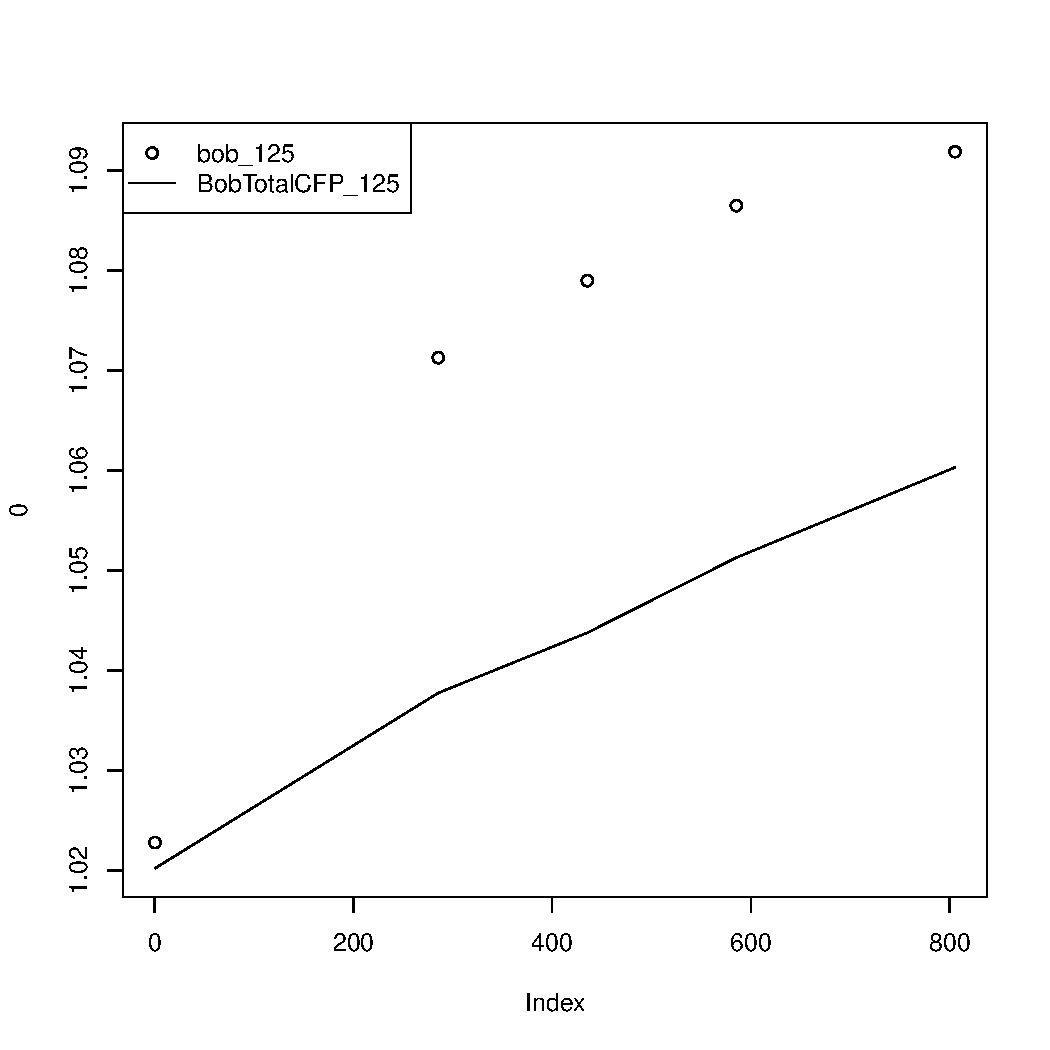
\includegraphics[width=10cm, height=7cm]{bob.pdf}
  \end{center}
 \end{frame}

 \begin{frame}{Solución}{Calibración según datos experimentales}

  Para las propiedades críticas y más propensas al error se efectúa una
  calibración de la correlación con base a datos experimentales.

  \begin{itemize}
   \item Un ajuste lineal de la correlación según su error con datos
	 experimentales.
	 
   \item Cada correlación ajustada es reinyectada para otros ajustes.
  \end{itemize}

 \end{frame}

\section{La técnica de calibración}

\begin{frame}{Ajuste lineal}
 
 \begin{columns}
  \begin{column}{5cm}
   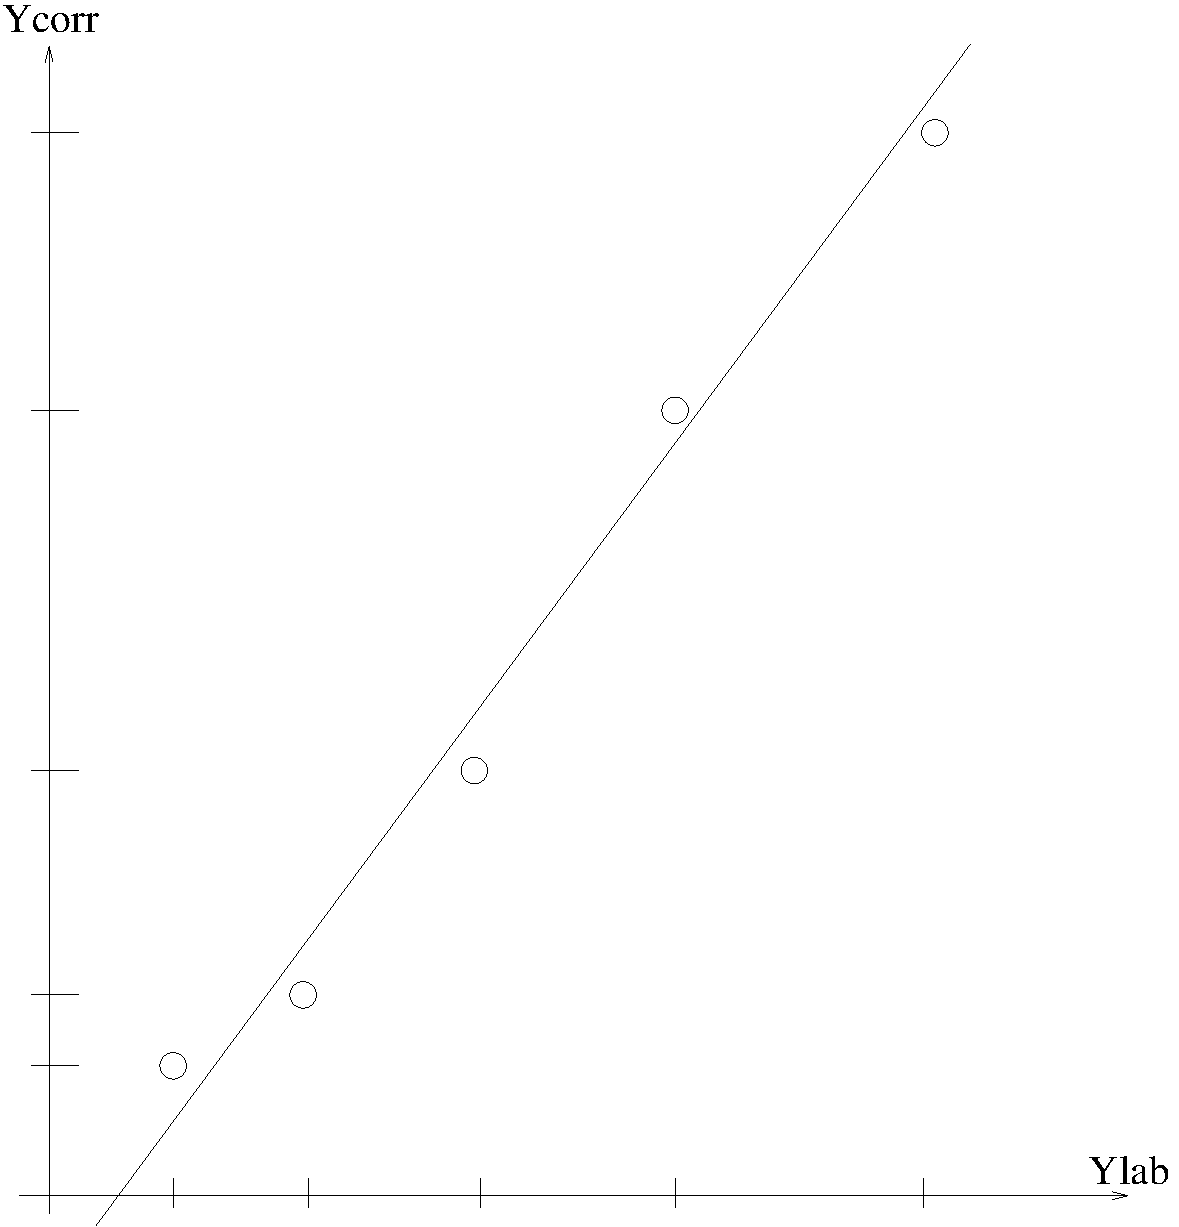
\includegraphics[scale=.25]{tuining}
  \end{column}
  \begin{column}{5cm}
   \begin{itemize}
    \item  Puntos experimentales ordenados por presión (sin
	  contar temperaturas).
    \item Regresión sobre el error obtiene recta    $Y_{ajusted} = c + m Y_{corr}$.

   \end{itemize}
      
   Indicadores para decidir:
    \begin{itemize}
     \item $R^2$, sumsq
     \item mse: suma de los errores al cuadrado.
     \item sigma ($\sigma$)
     \item $c$
     \item $m$
    \end{itemize}
  \end{column}
 \end{columns}
\end{frame}

\begin{frame}{Ejemplo con Bob calibrado}
 \begin{center}
  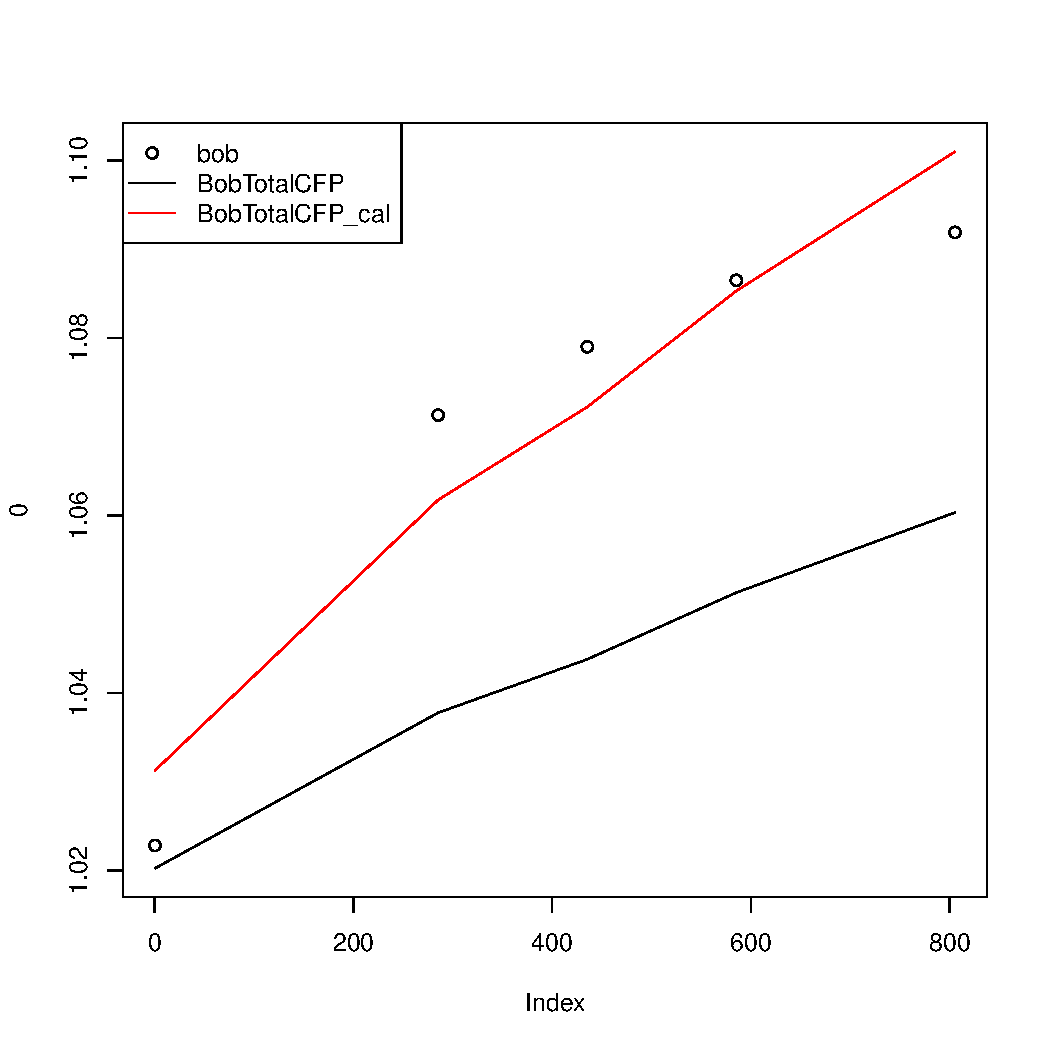
\includegraphics[width=10cm, height=7cm]{bob-cal}
 \end{center}
\end{frame}

\newcommand{\ttuner}{{\tt ttuner}\xspace}

\section{Backend ttuner}

\begin{frame}{\ttuner}
 
\ttuner es el nombre del backend que efectúa la calibración:

\begin{itemize}
 \item Todas las interacciones son por líneas de comandos.

 \item {\tt ./ttuner --help}: lista general de comandos.

 \item Otros backends:
       \begin{enumerate}
	\item {\tt cplot}: genera el grid.
	\item {\tt ztuner}: calibración automática del factor Z
       \end{enumerate}

 \item Backends desarrollados en C++.

 \item Diseñados para invocarse desde un front-end completamente independiente.

\end{itemize}
\end{frame}

\subsection{Entrada de datos}

\newcommand{\com}[1]{\textquotedbl #1\textquotedbl}

\begin{frame}{\ttuner: entrada de constantes}
 
Constantes: api, yg, rsb, n2, co2, h2s, psep, tsep, tsep2
\begin{itemize}
 \item {\tt ./ttuner --nom-constante valor}

 \item {\tt ./ttuner --api 10}

 \item {\tt ./ttuner --help: indica la unidad de entrada}m

\end{itemize}

Cambio de unidad: {\tt ./ttuner --unit \com{rsb Sm3/Sm3}}

\end{frame}

\begin{frame}{Entrada de vectores}

Propiedades experimentales se ingresan mediante vectores

\begin{itemize}
 \item rs: {\tt --rs\_data \com{tunit punit rsunit t pb pvals rsvals}}
 \item bob/boa: {\\t --bob\_data \com{tunit punit bobunit t pb bobp pvals bobvals}}
 \item coa: {\\t --coa\_data \com{tunit punit counit t pb pvals coavals}}
 \item uob/uoa: {\\t --uoa\_data \com{tunit punit uoaunit t pb uobp pvals uoavals}}
 \item uo:
\end{itemize}
\end{frame}

\subsection{split}

\subsection{Inputing}

\subsection{apply}

\subsection{napply}

\subsection{relax}

\subsection{split}

\subsection{Borrado de datos}

\end{document}


